
\documentclass[10pt]{article} % For LaTeX2e
\usepackage{tmlr}
% If accepted, instead use the following line for the camera-ready submission:
%\usepackage[accepted]{tmlr}
% To de-anonymize and remove mentions to TMLR (for example for posting to preprint servers), instead use the following:
%\usepackage[preprint]{tmlr}

% Optional math commands from https://github.com/goodfeli/dlbook_notation.
\input{math_commands.tex}

\usepackage{hyperref}
\usepackage{url}
\usepackage{booktabs}
\usepackage{tabularx}
\usepackage{tikz}
\usetikzlibrary{arrows.meta,calc,positioning,shapes.geometric}


\title{Tool-Lab: Tracing Information Acquisition and Optimal Decision-Making in Large Language Models}
% Opening the Black Box: Evaluating LLM Alignment through Process Tracing and Tool Use
% Authors must not appear in the submitted version. They should be hidden
% as long as the tmlr package is used without the [accepted] or [preprint] options.
% Non-anonymous submissions will be rejected without review.

\author{\name Davood Wadi \email davood.wadi@ucanwest.ca \\
      \addr University Canada West
      % \AND
      % \name Raia Hadsell \email raia@google.com \\
      % \addr DeepMind
      }

% The \author macro works with any number of authors. Use \AND 
% to separate the names and addresses of multiple authors.

\newcommand{\fix}{\marginpar{FIX}}
\newcommand{\new}{\marginpar{NEW}}

\def\month{MM}  % Insert correct month for camera-ready version
\def\year{YYYY} % Insert correct year for camera-ready version
\def\openreview{\url{https://openreview.net/forum?id=XXXX}} % Insert correct link to OpenReview for camera-ready version


\begin{document}


\maketitle

\begin{abstract}
Nothing
\end{abstract}

\section{Introduction}
% The Problem: LLMs are increasingly used for complex decision-making, but their internal information acquisition process remains opaque.
% The Inspiration: Introduce Mouselab and its historical significance in tracing human cognitive processes and information search.
% The Contribution: Introduce Tool-Lab, a novel methodology that adapts the Mouselab paradigm for LLMs by monitoring and analyzing their tool-calling behavior.
% Paper Outline: Briefly state what the subsequent sections will cover.

\section{Related Work}
% Tracing Human Decision-Making: Briefly discuss Mouselab, process tracing, and information acquisition in cognitive psychology and behavioral economics.
% LLM Decision-Making and Reasoning: Discuss current literature on LLM reasoning (e.g., Chain of Thought, ReAct) and evaluations of LLM behavior.
% Tool Use in LLMs: Review literature on how LLMs utilize external tools, APIs, and search functions, positioning Tool-Lab as a diagnostic method rather than just a capability enhancement.

% I need to create a table based on the research papers in mouselab directory in the repository, outlining all the research conducted so far in different disciplines.
% Columns: subject field, inline citation, brief experiment context, what was measured, what was found

\begin{table}[hbtp]
\centering
\caption{Summary of Mouselab research across disciplines.}
\small
\begin{tabularx}{\textwidth}{@{}p{2.5cm} p{2cm} X X X@{}}
\toprule
\textbf{Subject Field} & \textbf{Article} & \textbf{Context} & \textbf{Measures} & \textbf{Findings} \\
\midrule
Accounting \& Corporate Finance & \citet{hodge2004does} & Nonprofessional investors evaluated firms using searchable XBRL vs. PDF to allocate a \$10k investment. & Information acquisition and integration, investment decisions, and firm performance judgments. & XBRL technology improved nonprofessionals' acquisition and integration of disclosed information. \\
\addlinespace
Consumer Behavior & \citet{payne1988adaptive} & Simulated choice heuristics and human process-tracing using Mouselab evaluating risky multi-attribute options under time pressure. & Information acquisition (amount, speed, sequence, filtration) and relative choice accuracy. & Under high time pressure, users adapted by using attribute-based heuristics, processing faster, and filtering info, maintaining accuracy. \\
\addlinespace
Emotion \& Moral Psychology & \citet{luce1997choice} & Participants made multi-attribute choices under varying negative emotion conditions (e.g., child charity donation, job choice). & Extent and pattern of processing (time, sequence, alternative vs. attribute search), and self-reported emotion. & Higher negative emotion led to more extensive processing and a shift towards attribute-based, avoiding difficult trade-offs. \\
\addlinespace
Game Theory \& Behavioral Economics & \citet{johnson2002detecting} & Three-round sequential bargaining games with a shrinking pie to track information acquisition and backward induction. & Bargaining behavior (offers, rejection rates) and information search patterns (payoff box lookaheads). & Most subjects exhibited limited lookahead, failing backward induction; instruction improved both lookahead and normative offers. \\
\addlinespace
Healthcare Economics \& Policy & \citet{johnson2013can} \newline \citet{dellaert2024choice} & Consumers chose health insurance plans with/without aids (calculators, smart defaults); impacts of choice architecture. & Choice accuracy (cost-effectiveness), financial errors, weight on price components, and decision time. & Without decision aids, consumers made large financial errors by overweighting deductibles; smart defaults and calculators improved choices. \\
\addlinespace
Political Science & \citet{lau2006voters} & Voters gathered information and cast votes in a dynamic mock presidential election simulation with scrolling info. & Information search depth, comparability, sequence (candidate/attribute), and matching to decision strategies. & Voters vary in decision strategies (e.g., rational vs. heuristic); dynamic info tracking reveals heuristic use in complex races. \\
\addlinespace
Social Psychology \& Intergroup Bias & \citet{freeman2011looking} & Categorization of racially ambiguous faces dressed in high-status (business) vs. low-status (janitor) attire. & Categorization choice (White/Black) and real-time computer mouse hand trajectories (Area Under Curve). & High-status attire increased White categorizations, low-status increased Black; trajectories showed implicit attraction to unselected categories. \\
\bottomrule
\end{tabularx}
\end{table}

\section{The Tool-Lab Methodology}

Tool-Lab adapts process tracing to subjects whose only interface to the world is
linguistic and tool-mediated. Instead of watching a human participant move a
cursor over a visual decision board, we observe an LLM interacting through a
controlled action space: it can deliberate internally, call tools to inspect
currently available information, and emit text outputs such as intermediate
judgments or final choices. The experimental trace is therefore defined over
tool-mediated acquisitions and decisions rather than over mouse movements.
This preserves the core Mouselab idea that the order and extent of information
acquisition are themselves behavioral data.

Crucially, dynamic tasks need not be reduced to Payne-style static matrices in
order to be implemented for LLMs. The environment can maintain a latent state
and expose only the subset of cues that is currently available, updating that
state after each action. In this way, Tool-Lab can preserve transient cue
availability, missed-information costs, staged decisions, and other features of
dynamic tasks such as election campaigns, while still logging a clean and fully
structured action trace.

Resource scarcity can also be implemented directly in monetary terms. At the
start of an episode, the system prompt specifies a maximum budget $B$ (e.g.,
\$0.10). As the model reasons and invokes tools, the environment debits the
actual billed cost of model inference and tool execution under the prevailing
pricing schedule. This cost signal can be computed from observed usage without
recording the semantic contents of private reasoning. Each tool response then
returns not only the requested information, but also the marginal cost of that
action, cumulative expenditure, and the budget remaining. Monetary budget thus
serves as a domain-general implementation of search cost for LLM subjects,
playing the role that time pressure, effort, or access difficulty plays in
human process-tracing paradigms.

\section{Experiment 1: Political Science}
We instantiate the first Tool-Lab task as a dynamic presidential campaign adapted from
\citet{lau2006voters}. The original study asked human voters to navigate a mock election
in which information arrived as a transient stream rather than as a fixed table: only a
few candidate-attribute labels were visible at any moment, opening one item revealed its
contents, and the rest of the stream continued to move. This design is useful for
Tool-Lab because it turns information acquisition itself into the object of study. The
experiment does not ask only which candidate a model selects; it asks which pieces of
evidence the model decides are worth spending its limited access opportunities on. Because
the present paper focuses on the Tool-Lab methodology across multiple domains rather than
on reproducing every institutional feature of a single political study, we adopt the
simpler head-to-head general-election variant of the task.

Our environment preserves the core structure of the political-science task while
simplifying the electoral format. Each episode presents two unfamiliar presidential
candidates, one Democrat and one Republican, in a single general-election campaign.
Candidates are described through the same broad classes of cues emphasized by
\citet{lau2006voters}: issue positions, party and ideological labels, personal
background, personality cues, campaign strategy, endorsements, and polls. The model is
given a voter profile that includes political predispositions and can inspect only one
currently available item at a time.
Inspecting an item is implemented as a tool call. While the model reads that item, new
items continue to arrive and previously visible items can disappear, creating an explicit
opportunity cost for search. As in the original dynamic board, some cue types are
intentionally easier to encounter than others, allowing salient signals such as party and
poll standing to compete with more effortful issue-level evidence.

We log the full sequence of tool calls and evaluate the trace using three families of
measures from the Mouselab literature. Depth of search captures how much information the
model acquires before voting, measured from the number of unique items and distinct
attributes inspected. Comparability of search captures how evenly the model examines the
same attributes across the candidates in its current choice set. Sequence of search
captures whether the model searches candidate-by-candidate or attribute-by-attribute,
which allows us to distinguish more systematic compensatory search from shallower or
confirmatory heuristics. In the present single-election variant, these process measures
are computed over one campaign, which keeps the task compact while preserving the core
process-tracing logic of the original design.

Decision quality is evaluated separately from search behavior. Because the campaign is
synthetic, each candidate's attributes and the voter profile presented to the model are
fully specified in advance, which makes it possible to define a normative correct vote as
the candidate that best matches the fully informed preference profile. The
political-science experiment therefore yields two outputs for each model: a final vote and
a process trace. Comparing them lets us ask whether models that reach the correct choice
do so by broad, comparative search or by brittle heuristic shortcuts, and whether harder
campaign conditions, such as less ideologically distinctive matchups or tighter search
budgets, push models toward the same kinds of bounded strategies observed in human voters.

\subsection{Design}

At the level of experimental control, the political-science task is a synthetic
single general election with known ground truth. Each episode contains one Democratic and
one Republican candidate. Each candidate is instantiated from a common inventory of
forty-six candidate-specific attributes spanning issue positions, ideology, background,
personality, and campaign strategy, together with campaign-level cues such as
endorsements and polls \citep{lau2006voters}.
A voter profile is specified in advance and shown to the model at the start of the
episode, but the fully informed ranking that it induces over candidates is not. This
separation lets us score whether a model votes correctly without
confounding the benchmark with the model's own verbal rationale.

The model interacts with the campaign through a constrained inspection interface. During
the campaign, it can inspect only one currently available item at a time before deciding
whether to continue searching or cast its vote. To preserve the logic of the dynamic
information board, cue availability is transient: the visible window changes over time, some cue
types appear more frequently than others, and inspecting one item can cause other items
to be missed. Search therefore carries an explicit opportunity cost, rather than simply
revealing a fixed database in arbitrary order. In the LLM implementation, this
opportunity cost is made explicit through a monetary budget communicated in the
system prompt. Every reasoning step and tool invocation is charged at its
actual execution cost, and each tool result reports both the immediate charge
and the budget remaining.

The main manipulations target decision difficulty rather than institutional structure.
Following the original paradigm, we vary the ideological distinctiveness of the matchup
and, in some setups, the budget available for search, producing easier and harder
campaign conditions without changing the tool interface. All models are evaluated under
the same task specification and are compared on both outcome and process variables:
their vote, correctness relative to the fully informed benchmark, depth of search,
comparability of search, sequence of inspection actions, and resource expenditure. The
resulting design makes it possible to distinguish models that arrive at the same
electoral choice through systematic comparative search from models that reach that choice
through shallow or confirmatory heuristics.

\subsection{Procedure}

Each evaluation run is a single episode consisting of a briefing and one
general-election campaign. At the start of the episode, the model receives the
voter vignette and the rules of the inspection interface. The vignette defines
the goal of choosing the candidate
who best matches the assigned voter, but the fully informed ranking implied by
all hidden attributes is not revealed. From that point forward, the model can
interact only through the Tool-Lab actions: it may inspect one currently
visible item or stop searching and cast a vote. The prompt also states the
maximum spending budget for the stage, and every inspection returns not only
the newly revealed cue but also the marginal dollar cost of that action and the
budget that remains.

During the campaign, cue labels arrive in a rolling window and compete for
inspection. Opening a cue reveals one candidate- or campaign-level fact, but
because the stream continues to advance, other visible items can be missed
while the model is reading. The campaign ends when the model votes or when the
budget is exhausted. Any written justification is collected only after the vote
is recorded, so the process trace reflects pre-decision search rather than post
hoc explanation.

We repeat this procedure across multiple independent episodes for every
model-condition cell, covering both the easier and harder campaign conditions
described above. Candidate instantiations, cue order, and moment-to-moment
availability are randomized within the design constraints so that models cannot
solve the task by memorizing a fixed presentation order. Every action is logged
with its cue type, candidate target, and whether the information was new or
revisited. These logs are converted into the Mouselab measures of search depth,
comparability, and sequence for the single-election campaign, and the final vote
is scored against the fully informed benchmark. The resulting data pair outcome
quality with information-acquisition behavior for every run.

Figure~\ref{fig:political-science-procedure} summarizes the episode-level
procedure.

\begin{figure}[htbp]
\centering
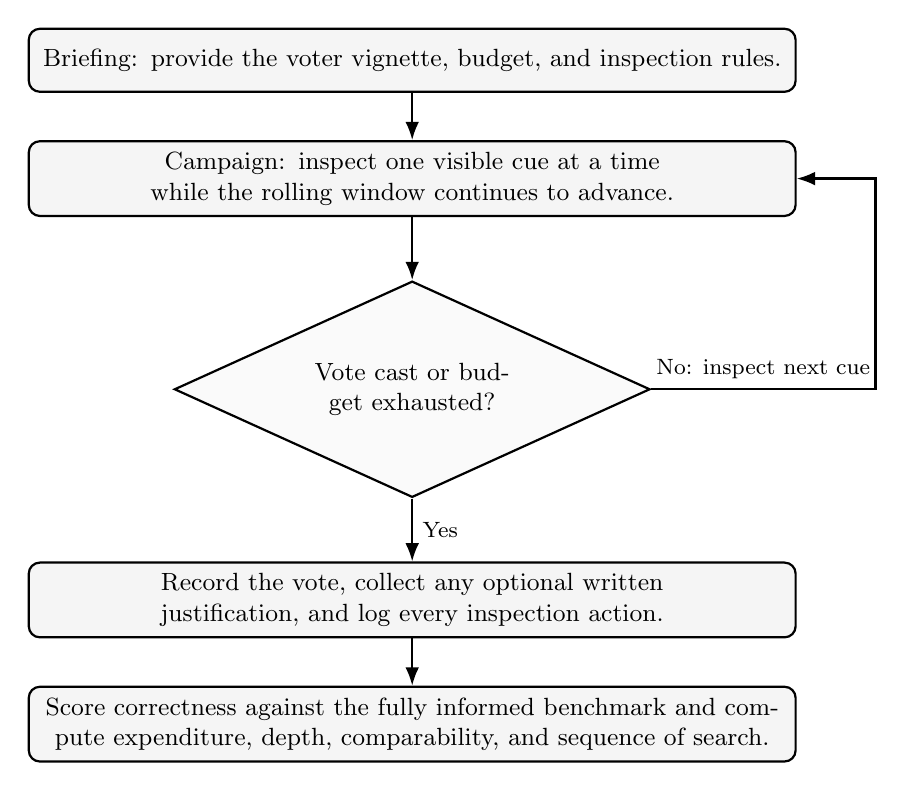
\begin{tikzpicture}[
      node distance=6mm,
      >=Latex,
      every node/.style={font=\small, align=center},
      process/.style={rectangle, rounded corners, draw, thick, fill=black!4,
            text width=0.78\linewidth, minimum height=8mm, inner sep=4pt},
      decision/.style={diamond, aspect=2.2, draw, thick, fill=black!2,
            text width=0.34\linewidth, inner sep=2pt},
      line/.style={->, thick}
]
\node[process] (brief) {Briefing: provide the voter vignette, budget,
and inspection rules.};
\node[process, below=of brief] (campaign) {Campaign: inspect one visible cue at a
time while the rolling window continues to advance.};
\node[decision, below=8mm of campaign] (stop) {Vote cast or budget exhausted?};
\node[process, below=8mm of stop] (post) {Record the vote, collect any optional
written justification, and log every inspection action.};
\node[process, below=of post] (score) {Score correctness against the fully informed
benchmark and compute expenditure, depth, comparability, and sequence of search.};
\coordinate (loop) at ([xshift=10mm]campaign.east);
\coordinate (loopreturn) at (loop |- stop.east);

\draw[line] (brief) -- (campaign);
\draw[line] (campaign) -- (stop);
\draw[line] (stop) -- node[right, font=\footnotesize] {Yes} (post);
\draw[line] (post) -- (score);
\draw[line] (stop.east) -- node[midway, above, font=\footnotesize]
      {No: inspect next cue} (loopreturn) -- (loop) -- (campaign.east);
\end{tikzpicture}
\caption{Tool-Lab political-science procedure for one evaluation episode.}
\label{fig:political-science-procedure}
\end{figure}

\subsection{Measures}

We evaluate each run at two levels: the quality of the vote that the model
ultimately casts and the process by which it acquires information before voting.
All measures are computed over the single election campaign, with the relevant
choice set defined as the two candidates on the ballot. Repeated openings of
the same cue are retained in the raw trace, but they count as revisits rather
than new information.

Because Tool-Lab is implemented over paid model inference and tool use, we also
measure resource expenditure directly. Each step in the trace records the
incremental dollar cost attributable to inference and tool execution, the
cumulative spend so far, and the budget remaining when the action completes. We
summarize these data as total spend, spend prior to the vote, and cost per
unique inspected cue, and we analyze decision quality conditional on
expenditure. These variables make the cost of search explicit and model-visible
rather than treating it as an unobserved latent constraint.

Depth of search measures how much information the model gathers before
stopping. Following \citet{lau2006voters}, we use three complementary
indicators so that the metric is not mechanically driven by the number of
candidates in the current choice set: (i) the number of distinct attributes
inspected at least once, (ii) the total number of unique cue items inspected for
candidates in the current choice set, and (iii) the average number of unique
cue items inspected per eligible candidate. For analysis, we report these
components directly and combine their within-stage standardized values into a
composite depth score. Higher values indicate broader and more persistent
search prior to voting.

Comparability of search measures whether the model compares like with like
across candidates rather than sampling idiosyncratic facts from each one. We
operationalize comparability at the attribute level. An attribute counts as
\emph{considered} if the model inspects it for at least one candidate in the
current choice set, and it counts as \emph{comparable} if the model inspects
that same attribute for every candidate in the set. The comparability score is
the proportion of considered attributes that become comparable by this
definition. A high score therefore indicates that the model is constructing
cross-candidate comparisons on common dimensions, whereas a low score
indicates patchier, less comparable search.

Sequence of search measures how the model moves from one inspection to the
next. Each adjacent pair of inspections is classified as candidate-based if the
model stays with the same candidate and switches attributes, attribute-based if
it keeps the same attribute and switches candidates, cross-switch if both
candidate and attribute change, or revisit if the identical cue is reopened.
Because our interface is dynamic and not every transition is always possible,
we normalize candidate-based and attribute-based search by the set of feasible
transitions at each step rather than by raw counts alone. This yields a
stage-specific candidate-based rate and attribute-based rate, together with a
signed orientation score defined as the difference between the two. Positive
values indicate a more candidate-based trace and negative values a more
attribute-based trace.

Outcome quality is evaluated independently of the process trace. For each
campaign, the environment defines a fully informed utility ranking over the two
eligible candidates from the assigned voter profile and the hidden cue values.
A vote is scored as correct if the model selects the candidate with the highest
fully informed utility; ties are treated as jointly correct. We report
correctness as a binary outcome and retain the full trace so that accurate
choices reached by systematic comparative search can be distinguished from
equally accurate choices reached by narrow heuristic search. This separation
between process and outcome is central to Tool-Lab: it lets us evaluate not
only whether a model reaches the right answer, but how it used its limited
inspection opportunities to get there.

\section{Experiment 2: Consumer Behavior}
% The Classic Problem: Describe the consumer choice scenario (e.g., choosing a product based on price, quality, and brand).
% Tool-Lab Adaptation: The specific tools provided (e.g., checking price, reading reviews).
% Results & Analysis: Analyze whether LLMs use compensatory vs. non-compensatory decision strategies, similar to human consumers.

\section{Experiment 3: Finance}
% The Classic Problem: Describe the financial scenario (e.g., portfolio selection, risk assessment, or evaluating corporate reports).
% Tool-Lab Adaptation: Tools provided (e.g., checking stock history, reading earnings summaries).
% Results & Analysis: Evaluate the risk tolerance, depth of financial search, and information overload handling of the various LLMs.

\section{Discussion and Insights}
% Cross-Domain Behavioral Patterns: What commonalities and differences exist in how different LLMs (e.g., GPT-5.4 vs. Claude 4.6) search for information? 
% LLMs vs. Humans: How does the tool-calling behavior of LLMs compare to the human behaviors documented in the original Mouselab studies?
% Implications for LLM Alignment: What do these information acquisition patterns tell us about how well these models are aligned with human reasoning and optimal decision-making?

\section{Conclusion and Future Work}
% Summary of the Tool-Lab methodology and the core findings from the three experiments.
% Limitations of the current study.
% Future directions for using Tool-Lab in other domains or for evaluating future generations of AI models.

\bibliography{main}
\bibliographystyle{tmlr}

\appendix
\section{Appendix}

\end{document}
